\begin{comment}
    \begin{itemize}
        \item Description of storm parameter clustering problem
        \item Introduction of variational inference
        \begin{itemize}
            \item Describe variational distribution
            \item Necessity (only model using t90 dataset)
            \item Relative performance (computational speed)
        \end{itemize}
        \item Describe clustering methodology
        \item Emergent clusters from both t90 and all--but--road--features in input space.
        \item What does this mean?
    \end{itemize}
\end{comment}

One potential application leveraging use of a Bayesian non-parametric prior is 
    exploiting the clustering inherent to the method. Recall $\delta_i$ is the 
    cluster identifier for observation $i$.  Its sampling is made explicit in
    the MCMC model, though it is integrated out in our variational model. In
    posterior analysis, given $\bm{\alpha}$, and $\bm{\pi}$, where 
    $\pi_j = \nu_j\prod_{k = 1}^{j-1}(1 - \nu_k)$, a probability of cluster 
    assignment can be sampled as
    \begin{equation}
        \label{eqn:clusterprob}
        \text{P}\left(\delta_i = j\mid\bm{\alpha},\bm{\nu},\bm{y}_i\right) 
            = \frac{\pi_j\mathcal{PG}(\bm{y}_i\mid\bm{\alpha}_j,\bm{1})}{
            \sum_{k = 1}^J \pi_j\mathcal{PG}(\bm{y}_i\mid\bm{\alpha}_k,\bm{1})}.
    \end{equation}
    This approach relies on samples of $\bm{\alpha},\bm{\nu}$ from the fitted
    model to generate \emph{loose} clusters for which there is no inherent 
    labelling.  This presents a problem, as interpreting clusters first requires
    \emph{labelling}, or a fixed assignment of observations to clusters.

The variational implementation avoids a label-switching issue inherent to 
    MCMC sampling.  A label-switch between clusters $a$ and $b$ has occured when
    the parameters of clusters $a$ and $b$ have nearly swapped, such that the
    bulk of observations formerly in cluster $a$ are now in cluster $b$, and 
    visa-versa.  This issue does not tend to follow to a variational 
    implementation, as post-fitting, the distributions of cluster parameters are 
    fixed.

With that being the case, a simple option for cluster labelling might be to take
    \[
        \bm{\alpha}_j^* = \frac{1}{S}\sum_{s = 1}^S\bm{\alpha}_{js}\hspace{2cm}
        \bm{\nu}_j^* = \frac{1}{S}\sum_{s = 1}^S \nu_{js},
    \]
    the posterior mean of cluster parameters and cluster weights, then set
    $\delta_i^{*} = \argmax P(\delta_i = j\mid\bm{\alpha}^*,\bm{\nu}^*,\bm{y}_i)$
    as defined in Equation~\eqref{eqn:clusterprob}. We refer to cluster labels
    being assigned in this fashion as \emph{posterior mean clustering}.

Alternative to posterior mean clustering, we could instead take samples of 
    $\bm{\pi}$, $\bm{\alpha}$, then compute 
    $\delta_{is}\mid\bm{\pi}_s,\bm{\alpha}_s$
    as per Equation~\eqref{eqn:clusterprob}.  Then set 
    $\delta_i^{*} = \argmax \mathbbm{1}_{\delta_{is} = j}$.
    We refer to cluster labels being assigned in this fashion as
    \emph{posterior assignment clustering}.  We find, in practice, this method
    results in largely the same label sets as posterior mean clustering.

























\subsection{Variational methods: a brief overview\label{ref:varbayes}}
\makenote{These 2 paragraphs are intended to introduce the justification for 
    VarBayes. I like the wordsmithing at the end of the second paragraph, but 
    I'm unsure of the necessity.  Specifically, the necessity of a generic 
    VarBayes intro as detailed here.}
Let $\bm{x}$ be the observed data, and $\bm{\theta}$ be an unobserved set of 
    parameters governing the distribution of the observed data.  We term 
    $f(\bm{x}\mid\bm{\theta})$ the likelihood.  The goal of inference in 
    general is to obtain information about $\theta$, using information 
    obtained from $\bm{x}$. Bayesian inference in particular places a prior
    distribution on $\theta$, $f(\bm{\theta})$, and from this we can obtain a
    posterior distribution on $\bm{\theta}$ that incorporates both information
    from the likelihood as well as the prior.  That is,
    \[
        f(\bm{\theta}\mid\bm{x}) = 
            \frac{f(\bm{x}\mid\bm{\theta})f(\bm{\theta})}{f(\bm{x})},
    \]
    where the demoninator $f(\bm{x})$ is obtained as
    \[
        f(\bm{x}) = \int_{\Omega_{\bm{\theta}}}f(\bm{x}\mid\bm{\theta})f(\bm{\theta})d\bm{\theta}
    \]
    where $\Omega_{\bm{\theta}}$ denotes the support of $\bm{\theta}$.

When a given model is sufficiently complex that the above integration is no
    longer feasible analytically, or if the posterior cannot be described in
    closed form\makenote{when the posterior is not tractible...}, we frequently 
    turn to sampling--based classes of methods, such as 
    \emph{Markov chain Monte Carlo} (MCMC)\needcite. There are myriad approaches, 
    \makenote{expand?}, but central to all sampling--based 
    methods is the stochastic nature of model fitting, and the 
    necessity of samples for posterior inference.  Sampling methods can be 
    tempermental, requiring many numbers of iterations to reach convergence.
    Samples take time to draw, and memory to store; but for sufficiently large 
    problems, both can be in short supply.

One class of methods that shows promise in avoiding the computational and 
    storage burdens of sampling methods is variational inference.\needcite 
    Based on variational calculus, this approach attempts to approximate the 
    true posterior distribution
    $f(\bm{\theta}\mid\bm{x})$ using a tractible \emph{surrogate posterior} 
    $q(\bm{\theta})$.  Model fitting under this class involves specification of 
    the family of surrogate densities $\mathcal{Q}$, then selecting that density 
    $q^*$ which minimizes the \emph{Kullbeck-Liebler} (KL) divergence between 
    the surrogate and true posterior.  That is,
    \begin{equation}
        \label{eqn:optimalq}
        q^*(\bm{\theta}) = \argmin_{q\in\mathcal{Q}}\left\lbrace
        \text{KL}\left(q(\bm{\theta})||f(\bm{\theta}\mid\bm{x})\right) 
        \coloneqq
        \text{E}_{q}\left[\log\left(
        \frac{q(\bm{\theta})}{f(\bm{\theta}\mid\bm{x})}
        \right)\right]
        \right\rbrace.
    \end{equation}
    Using KL divergence as an analogue to distance, we are attempting to find
    the \emph{closest} tractable surrogate posterior $q$ within the family 
    $\mathcal{Q}$ to the true posterior.  
    As has been explained however, we do not necessarily have 
    $f(\bm{\theta}\mid\bm{y})$ directly.  Let 
    $f(\bm{y},\bm{\theta}) = f(\bm{y}\mid\bm{\theta})f(\bm{\theta})$.
    Then we reformulate the KL divergence into
    \[
        \begin{aligned}
        \text{KL}\infdiv{q(\bm{\theta}\mid\bm{\psi})}{f(\bm{\theta}\mid\bm{x})}
            &=\text{E}_{\bm{\psi}}\left[\log\left(
                \frac{q(\bm{\theta}\mid\bm{\psi})}{f(\bm{\theta}\mid\bm{x})}
                \right)\right] = \text{E}_{\bm{\psi}}\left[
                \log\left(\frac{q(\bm{\theta}\mid\bm{\psi})f(\bm{x})}{f(\bm{y},\bm{\theta})}
                \right)\right]\\
            &= \text{E}_{\bm{\psi}}\left[
                \log q(\bm{\theta}\mid\bm{\psi}) - \log f(\bm{x},\bm{\theta}) 
                + \log f(\bm{x})
                \right]\\
            &= \text{E}_{q}\left[
                \log q(\bm{\theta}) - \log f(\bm{x},\bm{\theta})\right] + 
                   \log f(\bm{x}).
        \end{aligned}
    \]
    Note that the second term, the \emph{evidence}, is constant with respect to 
    $\bm{\theta}$.  With a bit of rearrangement,
    \[
        \begin{aligned}
        \log f(\bm{x}) 
            &= \text{KL}\infdiv{q(\bm{\theta})}{f(\bm{\theta}\mid\bm{x})}
                - \text{E}_q\left[
                \log q(\bm{\theta}) - \log f(\bm{x},\bm{\theta})
                \right]\\
            &= \text{KL}\infdiv{q(\bm{\theta})}{f(\bm{\theta}\mid\bm{x})}
                + \mathcal{L}(\bm{\theta})
        \end{aligned}
    \]
    Thus maximizing $\mathcal{L}(\bm{\theta})$ is equvivalent to minimizing the 
    KL divergence. In this form, as KL divergence is a positive quantity, it is
    readily apparent that $\mathcal{L}(\bm{\theta})$ establishes a lower bound
    on the evidence.  As such, the variational literature has christened it the
    \emph{evidence lower bound}, often abbreviated to \emph{ELBO}.  As such,
    we can rewrite Equation~\eqref{eqn:optimalq} to
    \[
        q^*(\bm{\theta}) = \argmax_{q\in\mathcal{Q}} \mathcal{L}(\bm{\theta})
    \]
    Note that we specify $q$ so as to depend on a set of variational parameters 
    $\bm{\psi}$, such that choosing the optimal $\bm{q}$ means in effect choosing
    the optimal $\bm{\psi}$.  

Optimization of the ELBO with respect to $\bm{\psi}$ can be a daunting task.
    If $q$ is specified in such a way that samples of $\bm{\theta}$ can be 
    generated as a function of $\bm{\psi}$ and some independent random variable 
    $\epsilon$ such as $\psi_0\epsilon + \psi_1$ as in the case of a normal
    random variable, then given samples of $\bm{\theta}$ we can differentiate 
    the ELBO with respect to $\bm{\psi}$ to calculate the gradient of $\bm{\psi}$
    at the current value.  Using this gradient, we can iteratively move towards
    a better position---a more optimal $\bm{\psi}$.

That said, a path-based optimization is highly dependent upon the starting position,
    and if multiple local optima exist, there is no guarantee we will reach the
    true optimal value.  There are many approaches that seek to solve this issue,
    such as stochastic gradient descent, simulated annealing, \makenote{add additional algorithms}
    but the problem remains.  Even in our testing, using what is well regarded as
    one of the best optimization algorithms available, our results are still
    highly dependent upon starting position, both in terms of model fidelity, and
    in terms of the resulting number of extant mixture components.  That said, 
    another approach we can consider is finding a better starting position.

\subsection{Optimal starting position}

As we are considering a mixture model where potentially there exists a label switching
    issue, if the initializing distribution of mixture component parameters provides
    \emph{decent} coverage of the distribution of optimal parameters, then the most 
    important part of the initialization is the distribution of mixture \emph{weights}.  
    Here we consider three strategies.  First is, of course, random initialization.  
    Second is uniform initialization---initializing the parameters such that, after
    transformation via stick-breaking, the probability of cluster assignment is uniform
    among all clusters up to the truncation point.  Finally, we can declare a rather
    optimistically named \emph{optimal} starting point as a result of using an abridged
    MCMC sampler solely for cluster assignments, then after some number of iterations,
    declaring the full conditional distribution of the resultant mixture weights and
    associated parameters as the starting point for the VB algorithm.

\begin{figure}[b]
    \caption{Rise in energy score over baseline by number of dimensions, on simulated data for various model fitting strategies. The faceting denotes the number of mixture components in
    the generating distribution. \label{fig:energyscore}}
    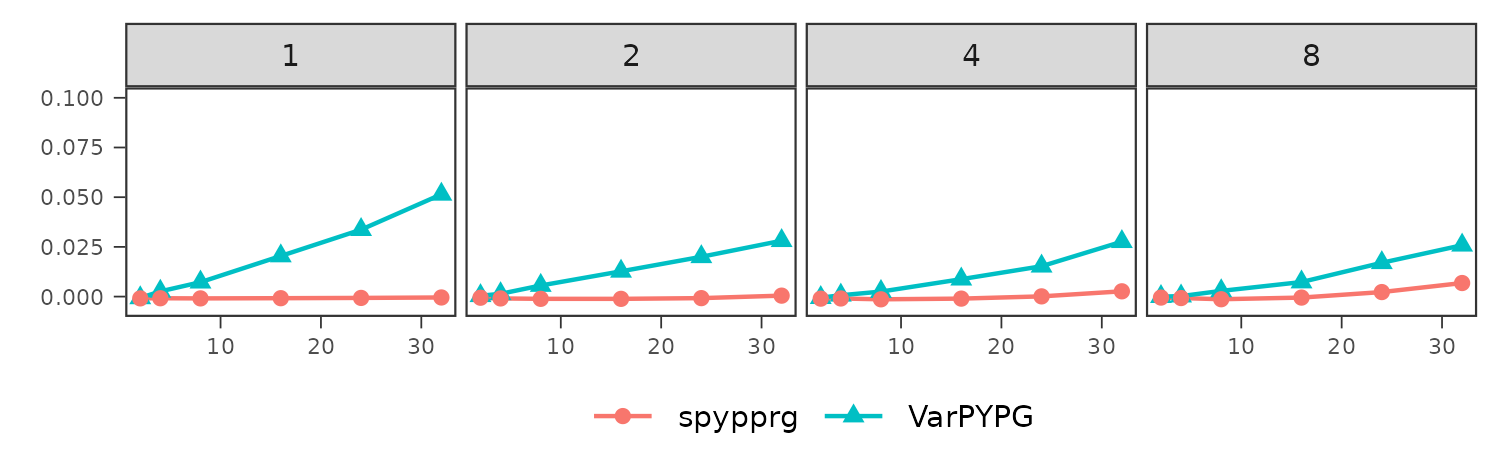
\includegraphics[width=\linewidth]{plots/energy_score}
\end{figure}

Figure~\ref{fig:energyscore} displays the results of our foray looking into this 
    optimal starting position, by examining the rise in energy score calculated from a
    posterior predictive sample over a baseline energy score calculated from
    another random sample from the same generating distribution.  We see that a pure 
    MCMC approach performs best, but using an abridged MCMC sampler to set a 
    starting position for the variational algorithm performs nearly as well.  It is
    also much faster \makenote{this needs to be quantified}.

% EOF